\documentclass{article}


% Packages
\usepackage[utf8]{inputenc} % Encoding support
\usepackage[T1]{fontenc} % Better font rendering
\usepackage{amsmath, amssymb} % Math support
\usepackage{geometry} % Page layout
\geometry{a4paper, margin=1in}
\usepackage{graphicx} % For including images
\usepackage{xcolor} % Color support
\usepackage{hyperref} % Clickable links in the document
\usepackage{caption} % Custom captions for figures and tables
\geometry{a4paper, margin=1in}

% Title and Author
\title{Gradient based PCQA}

\date{\today}

\begin{document}

\maketitle


\section{Idea}

To check whether a point or a neighborhood of points are good quality, we want use the gradient of the point cloud together with individual points. The quality of the points will be determined by a Neural Network that we will train on different features. The neural network will be designed to determine an radius of a Euclidean ball and how many points should be inside this radius. Both the radius and k-number of points inside will be based on several features including the gradient. If the number of points inside the Euclidean ball is less than the number of points determine there should be by the Neural Network, then the point i marked as "bad" and need a re-scan.
\begin{figure}[h]
    \centering
    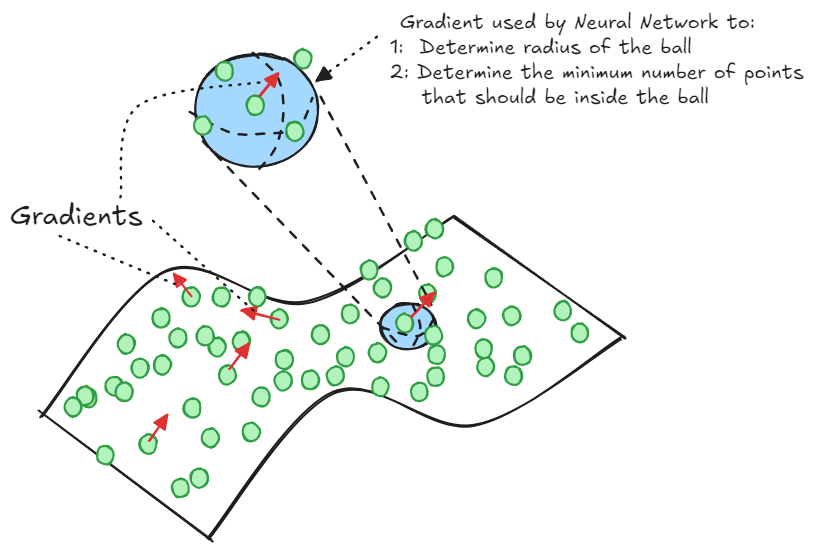
\includegraphics[width=0.8\linewidth]{Idea3D.png}
    \caption{3D visualization of the idea}
    \label{fig:3didea}
\end{figure}



\section{Neural network: features and outputs}
Possible features that could be used as inputs:
\begin{itemize}
    \item Gradient
    \item Curvature 
    \item ...
\end{itemize}

The output should be a quality assessment of the point together with a confidence score of the output.




\subsubsection*{Possible error handling:}
This is a maybe, just some thoughts\\
If the neural network gives out a low confidence score, mark the area as "undefined" and maybe run some local areas with the regular PCQA method.


\end{document}



































